\documentclass[11pt,a4paper]{article}
\usepackage{fontspec}
\setmainfont{TeX Gyre Termes}
\setmonofont{Latin Modern Mono}[Scale=0.95]
\usepackage[margin=2.6cm,top=2.8cm,bottom=2.8cm]{geometry}
\usepackage{graphicx,booktabs,amsmath,xcolor,listings,fancyhdr,caption,titlesec,microtype,enumitem}
\usepackage[hidelinks]{hyperref}
\usepackage{float}
\usepackage[round,authoryear]{natbib}

\definecolor{codebg}{HTML}{F5F5F2}
\definecolor{codekw}{HTML}{1C5CAB}
\definecolor{codecm}{HTML}{6E6D68}
\lstset{language=Python,basicstyle=\ttfamily\small,backgroundcolor=\color{codebg},
  keywordstyle=\color{codekw},commentstyle=\color{codecm}\itshape,
  frame=none,xleftmargin=1em,framexleftmargin=1em,aboveskip=8pt,belowskip=8pt,
  columns=fullflexible,keepspaces=true,showstringspaces=false}

\captionsetup{font={small,it},labelfont={small,it},justification=centering}
\titleformat{\section}{\large\bfseries}{\thesection.}{0.5em}{}
\titleformat{\subsection}{\normalsize\bfseries}{\thesubsection}{0.5em}{}
\titlespacing*{\section}{0pt}{14pt}{6pt}
\titlespacing*{\subsection}{0pt}{10pt}{4pt}
\setlength{\parskip}{5pt}\setlength{\parindent}{0pt}

\pagestyle{fancy}\fancyhf{}
\fancyhead[L]{\small\itshape Credit Risk in Germany}
\fancyhead[R]{\small\itshape Ettore Mancuso}
\fancyfoot[C]{\small\thepage}
\renewcommand{\headrulewidth}{0.4pt}\renewcommand{\footrulewidth}{0.4pt}

\begin{document}
\thispagestyle{empty}
\begin{center}
{\LARGE\bfseries Credit Risk in Germany:\\[4pt] From System-Wide Signals to a Borrower-Level PD Model}\\[10pt]
{\large\itshape Insolvencies, bank asset quality, default prediction and\\ what the resulting PDs mean for capital under the CRR}\\[22pt]
{\large Ettore Mancuso}\\[1pt]
\href{mailto:ettoremancuso6@gmail.com}{ettoremancuso6@gmail.com}\\[1pt]
October 2026
\end{center}
\vspace{16pt}

\section*{Abstract}
For about ten years German banks lost very little money on bad loans. That period is ending, and I look at it from two sides. At the level of the system, I put together a small, fully sourced dataset from Destatis, the EBA, the ECB, BaFin and the Bundesbank. Corporate insolvencies reached 24,064 in 2025, 72\% above their 2021 trough and the second-highest count since 2013. The stock of non-performing loans rose from EUR~29.7 to 48.6 billion between 2021 and 2025, and the share of loans in IFRS~9 Stage~2 is 15.3\%, against 8.9\% for the EU. At the level of the borrower, I estimate Probability of Default (PD) models on the German Credit data, 1,000 consumer loans from a southern German bank. A Weight-of-Evidence logistic scorecard reaches a test AUC of 0.80 and does as well as a random forest and gradient boosting, while staying fully readable. I then map the scorecard into seven rating grades and run the PDs through the CRR risk-weight function for retail exposures. With a 3\% portfolio PD and a 45\% LGD, the IRB approach needs 71\% of the capital of the standardised approach, so the output floor would not bind at its 2025 level of 50\% but would bind once it reaches 72.5\% in 2030. All code and data are public.

\medskip
\textbf{Keywords:} credit risk, probability of default, logistic regression, credit scoring, machine learning, IRB approach, CRR3, output floor, non-performing loans, Germany

\textbf{JEL classification:} G21, G28, G32, C25, C53

\section{Introduction}
For most of the 2010s German banks had an easy credit cycle. Interest rates were low, unemployment fell and corporate insolvencies declined almost every year, reaching a low of 13,993 in 2021 \citep{destatis2023}. Since then things have changed. Three years of weak growth, higher rates and a correction in commercial property have pushed insolvencies back above their pre-pandemic level \citep{destatis2026}, and the Bundesbank now describes a non-performing loan ratio that has ``risen steadily since the end of 2022'', starting in commercial real estate and spreading to other sectors \citep{bbk2025}.

Credit risk can be studied from the top, through aggregate indicators, or from the bottom, through the models that banks use to price and approve individual loans. Students usually meet the two in different courses. In this project I try to connect them. The questions are:

\begin{enumerate}[leftmargin=1.5em,itemsep=2pt]
\item What do official data say about the direction of credit risk in the German banking system, and how does Germany compare with the rest of the EU?
\item With borrower-level data, how well can a simple, transparent PD model predict default, and do machine-learning methods do better?
\item What do those PDs imply for regulatory capital under the Capital Requirements Regulation (CRR), including the output floor introduced by CRR3?
\end{enumerate}

Section~2 summarises the regulatory framework. Section~3 describes data and methods, Section~4 presents the results, Section~5 discusses them, Section~6 lists the limitations and Section~7 concludes. Every number, table and figure comes from a Jupyter notebook in the accompanying repository, which also contains an SQL file for the segment analysis and an R script that cross-checks the logistic model.

\section{Regulatory background}
Under the CRR \citep{crr}, a bank can compute capital for credit risk with the standardised approach, which assigns fixed risk weights by exposure class (75\% for regulatory retail exposures, Art.~123), or, with supervisory approval, with the internal ratings-based (IRB) approach. Under IRB, the bank estimates the PD of each borrower and, for retail, also the loss given default (LGD) and the exposure at default (EAD). The regulation turns these inputs into capital through the Vasicek one-factor model. For an \textit{other retail} exposure the capital requirement per unit of EAD is
\begin{equation}
K = \text{LGD}\cdot\Phi\!\left(\frac{\Phi^{-1}(\text{PD})+\sqrt{R}\,\Phi^{-1}(0.999)}{\sqrt{1-R}}\right)-\text{PD}\cdot\text{LGD},
\end{equation}
where $\Phi$ is the standard normal distribution and the asset correlation $R$ falls from 16\% to 3\% as PD rises \citep[Art.~154]{crr}. The first term is the loss rate in a one-in-a-thousand-year downturn; subtracting expected loss leaves the unexpected part, which capital has to absorb \citep{bcbs2005}. The risk weight is $12.5K$.

CRR3 \citep{crr3}, which has applied since January 2025, keeps this formula but limits how low internal estimates can go. PDs cannot be set below 0.05\%, foundation-IRB LGDs for senior unsecured corporate exposures fall from 45\% to 40\%, and, most importantly, the output floor caps the benefit of internal models: total risk-weighted assets cannot be lower than a percentage of what the standardised approach would give, rising from 50\% in 2025 to 72.5\% in 2030 \citep{pwc_crr3}.

\section{Data and methods}
\subsection{System-level data}
No single database tracks credit risk in German banks across all the dimensions I need, so I collected the values by hand. Every row in the data files records its source (Table~\ref{tab:data}). The insolvency series is complete for 2010--2025. The banking indicators are point observations rather than long series: the EBA and ECB country data are published as dashboards and statistical tables that change sample and definition over time, and I preferred a few comparable figures to a long series that mixes definitions.

\begin{table}[H]\centering\small
\caption{System-level data used in the analysis.}\label{tab:data}
\begin{tabular}{p{4.4cm}p{4.7cm}p{4.6cm}}
\toprule
File & Content & Sources \\
\midrule
\texttt{insolvencies\_de.csv} & Corporate insolvencies, 2010--2025 & \citet{destatis2023}; \citet{destatis2026} \\
\texttt{npl\_indicators.csv} & NPL ratios (total, corporate, commercial real estate), Stage~2 shares, NPL stock, CET1 and return on equity & EBA Risk Dashboard via \citet{bks2026a,bks2026b}; \citet{bafin2026}; \citet{ecb2026} \\
\texttt{regulation\_parameters.csv} & Risk-weight parameters, floors, output-floor schedule & \citet{crr}; \citet{crr3}; \citet{pwc_crr3} \\
\bottomrule
\end{tabular}
\end{table}

\subsection{Borrower-level data}
Banks do not publish loan-level data, so the borrower-level analysis uses the German Credit data \citep{hofmann1994}: 1,000 consumer loans from a southern German bank, each with 20 attributes (account balances, credit history, purpose, amount, duration, employment, housing and so on) and a good/bad label. Most published credit-scoring studies use it, so my results can be checked against theirs. It also has two problems I need to deal with.

First, the widely circulated version contains coding errors. \citet{groemping2019} reconstructed the original codes and showed that several category labels are wrong. I therefore treat the categories as anonymous groups and do not draw conclusions from their labels. Second, 30\% of the loans are bad, far more than in any real consumer portfolio, because defaults were over-sampled. The models only need to rank borrowers, so this is not a problem for estimation; before computing capital, however, I shift the PDs to a realistic level (Section~3.4).

I drop two attributes, the combined sex and marital status variable and the foreign-worker flag. Sex and nationality should not drive a credit decision, and creditworthiness scoring of natural persons is classified as a high-risk use under the EU AI Act \citep{aiact}. The remaining 18 attributes enter the models.

\subsection{Models and validation}
The data are split into a training set (70\%) and a test set (30\%), stratified by outcome. I estimate three models:

\begin{enumerate}[leftmargin=1.5em,itemsep=2pt]
\item a \textbf{logistic scorecard}: each attribute is binned and replaced by its Weight of Evidence, $\text{WoE}=\ln(\%\text{good}/\%\text{bad})$, and attributes with an Information Value below 0.02 are discarded \citep{siddiqi2006};
\item a \textbf{random forest} with 500 trees;
\item \textbf{gradient boosting} with 300 shallow trees.
\end{enumerate}

The WoE bins are fitted on training data only, and inside each cross-validation fold, so that no information from the validation data leaks into the encoding. I compare the models with five-fold cross-validated AUC on the training set and with AUC, Gini, the Kolmogorov--Smirnov statistic and the Brier score on the test set. As a cross-check, an R script fits a plain logistic regression with dummy-coded categories on the same split.

\subsection{From PD to rating grades and capital}
To grade the whole portfolio without in-sample bias, each loan receives an out-of-fold PD from five-fold cross-validation. I then shift the intercept of the log-odds until the average PD equals 3\%. This keeps the ranking unchanged and only moves the level. The 3\% is an assumption for a consumer-loan book, not a feature of the data, so I also report results at 2\% and 5\%. Loans are assigned to seven grades, A to G, with PD bands that roughly double at each step, which is how many banks build their master scale. For capital, EAD is the loan amount and LGD is 45\% in the baseline and 30\% in the sensitivity; the data contain no recovery information. The risk-weight function in the repository is a direct translation of equation (1):

\begin{lstlisting}
def other_retail_correlation(pd_):
    w = (1 - np.exp(-35 * pd_)) / (1 - np.exp(-35))
    return 0.03 * w + 0.16 * (1 - w)

def risk_weight(pd_, lgd):
    pd_ = np.maximum(pd_, 0.0005)          # CRR3 PD floor for retail
    r = other_retail_correlation(pd_)
    stressed_pd = norm.cdf((norm.ppf(pd_) + np.sqrt(r) * norm.ppf(0.999))
                           / np.sqrt(1 - r))
    return 12.5 * (lgd * stressed_pd - lgd * pd_)
\end{lstlisting}

\section{Results}
\subsection{The credit cycle has turned}
Figure~\ref{fig:ins} shows corporate insolvencies since 2010. The long decline ended in 2021, when government support and the temporary suspension of the duty to file kept many firms alive. Since then the count has risen by 22\% in 2023, 22\% in 2024 and 10\% in 2025, to 24,064 cases, 28\% above 2019 and only 21 cases short of 2014 \citep{destatis2026}. Insolvency rates are highest in transport, hospitality and construction.

\begin{figure}[htbp]\centering
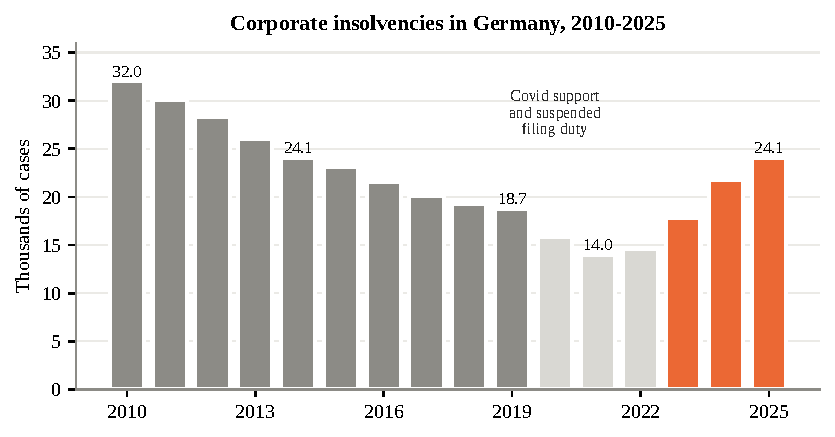
\includegraphics[width=0.86\textwidth]{../figures/fig1_insolvencies.pdf}
\caption{Corporate insolvencies in Germany. Light grey bars mark the pandemic years; orange bars the increase since 2023. Source: Destatis.}\label{fig:ins}
\end{figure}

Bank balance sheets show the same turn with a lag. The stock of non-performing loans at German banks went from EUR~29.7 billion at the end of 2021 to EUR~48.6 billion at the end of 2025, an increase of 64\% \citep{bks2026b}. Figure~\ref{fig:npl} puts Germany next to the EU. The headline NPL ratio, 1.61\%, is still below the EU average of 1.82\%, but it is the highest in Germany since 2018 and it is moving the other way: the EU ratio is falling \citep{bks2026a}. The clearest case is commercial real estate. In 2019 German banks had a CRE NPL ratio of 1.7\% against 8.6\% in the EU; by the end of 2025 the positions had reversed, at 6.9\% against 4.1\%. The Stage~2 share, loans whose credit risk has increased significantly since origination, is 15.3\% in Germany and 8.9\% in the EU. Stage~2 loans are the ones most likely to turn into NPLs next, so I find this gap more worrying than the headline ratio. For corporate loans as a whole, BaFin reports an NPL ratio of 3.8\% in the third quarter of 2025, higher at smaller banks (4.26\%) than at significant institutions (3.66\%) \citep{bafin2026}.

\begin{figure}[htbp]\centering
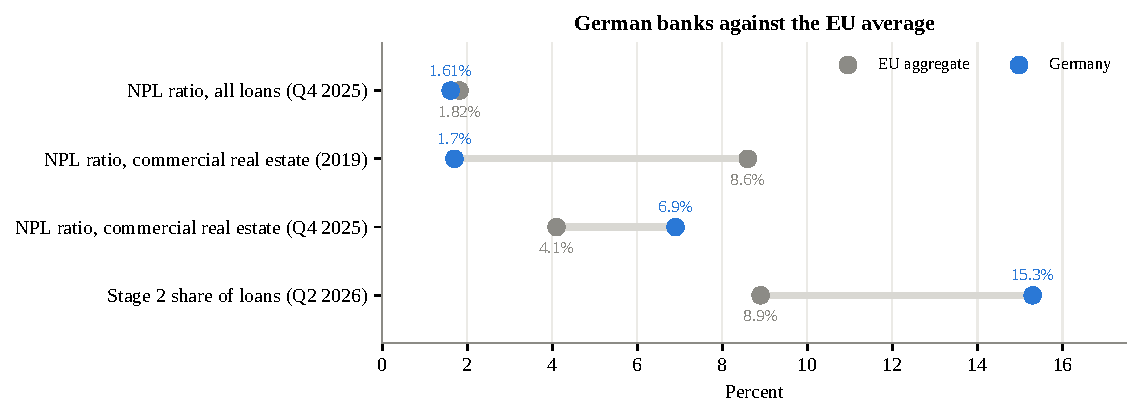
\includegraphics[width=0.86\textwidth]{../figures/fig2_npl_compare.pdf}
\caption{Asset-quality indicators, German banks against the EU aggregate. Sources: EBA Risk Dashboard, as reported by BKS e.V.}\label{fig:npl}
\end{figure}

German banks enter this phase with capital ratios that the Bundesbank calls high, but also with the lowest profitability among large euro-area banks: a return on equity of 6.38\% at the end of 2025, against 9.53\% for the euro area \citep{ecb2026}. The Bundesbank adds a warning that is directly relevant to the second part of this paper: risk weights at the systemically important banks remain low despite the worse risk picture, so capital ratios may overstate resilience \citep{bbk2025}. Those risk weights are produced by PD models like the ones in the rest of this paper, which is why I move from aggregate data to individual loans.

\subsection{What predicts default}
Even simple SQL queries on the loan data show large differences between groups. Borrowers with a negative checking-account balance default in 49.3\% of cases, those without a checking account at this bank in 11.7\%. Default rates rise steadily with the length of the loan, from 21.2\% for up to one year to 51.7\% beyond three years, and long loans are also much larger on average (DM~7,646 against DM~1,811). Figure~\ref{fig:iv} ranks all 18 attributes by Information Value. Checking-account status is by far the strongest (IV 0.63), followed by credit history, savings and duration. Four attributes carry almost no information, among them the number of dependants and the length of residence, and are dropped from the scorecard, which keeps 14.

\begin{figure}[htbp]\centering
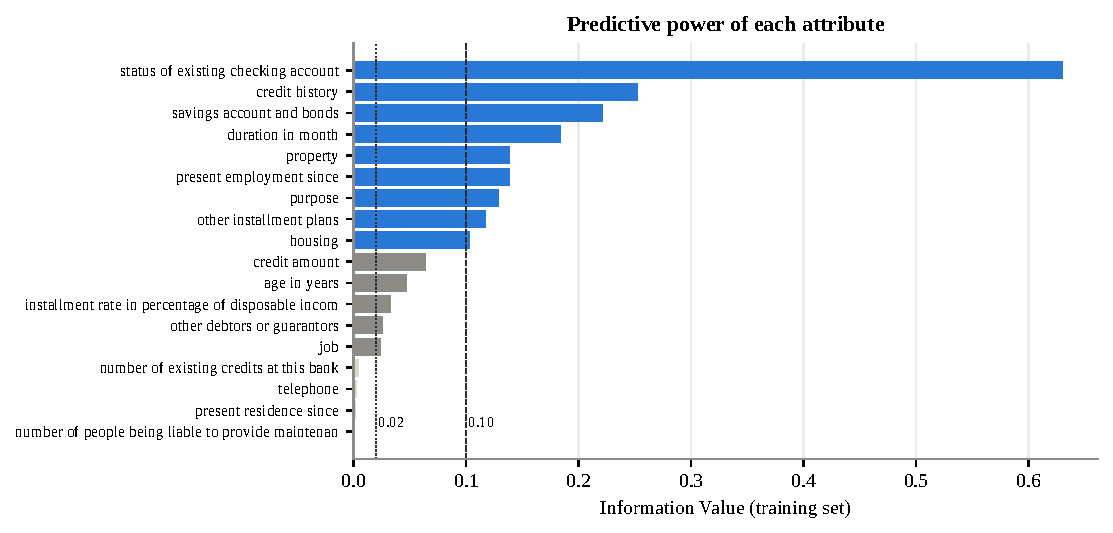
\includegraphics[width=0.84\textwidth]{../figures/fig3_iv.pdf}
\caption{Information Value of each attribute on the training set. Dotted line: 0.02, below which an attribute is discarded; dashed line: 0.10, the conventional threshold for medium predictive power.}\label{fig:iv}
\end{figure}

\subsection{Logistic regression holds its own}
Table~\ref{tab:models} compares the three models. On the test set they are practically tied: AUC between 0.794 and 0.801, Gini around 0.6. The random forest has the best cross-validated AUC (0.783), but also the largest variance across folds and the worst Brier score. With 300 test loans, differences of 0.01 in AUC are well within sampling noise. The R cross-check, a logistic regression on dummy-coded categories, reaches a test AUC of 0.792, close to the scorecard.

\begin{table}[H]\centering\small
\caption{Model comparison. CV: five-fold cross-validation on the training set (n = 700); test set n = 300.}\label{tab:models}
\begin{tabular}{lcccccc}
\toprule
Model & CV AUC & CV s.d. & Test AUC & Gini & KS & Brier \\
\midrule
Logistic scorecard (WoE) & 0.758 & 0.019 & 0.801 & 0.601 & 0.502 & 0.159 \\
Random forest & 0.783 & 0.035 & 0.794 & 0.587 & 0.481 & 0.166 \\
Gradient boosting & 0.764 & 0.019 & 0.796 & 0.592 & 0.462 & 0.159 \\
\bottomrule
\end{tabular}
\end{table}

\begin{figure}[htbp]\centering
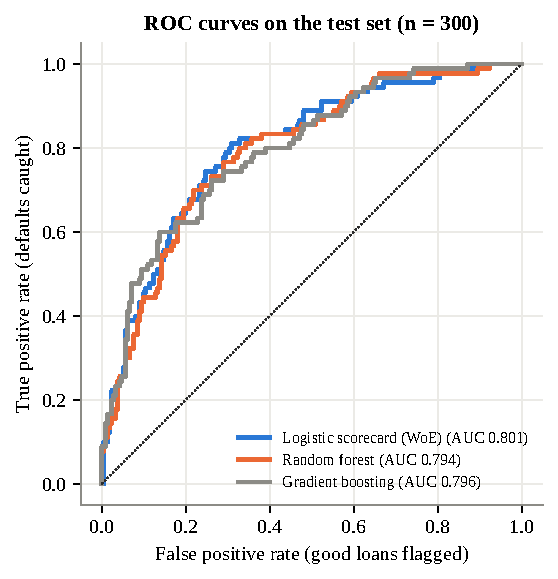
\includegraphics[width=0.62\textwidth]{../figures/fig4_roc.pdf}
\caption{ROC curves of the three models on the test set.}\label{fig:roc}
\end{figure}

What the table does not show is that the scorecard can be read line by line. In an unpenalised logit on the WoE variables, 13 of the 14 coefficients have the expected negative sign (a safer bin lowers the odds of default), and the only exception, job type, is far from significant ($p=0.33$). A credit officer can explain every decision, and a supervisor can check every variable. \citet{lessmann2015} found something similar across many credit datasets: on small tabular data, advanced classifiers rarely beat a well-built logistic model by much.

\subsection{Rating grades}
Table~\ref{tab:grades} and Figure~\ref{fig:grades} show the master scale. The grades separate risk well: in the sample, the observed default rate rises monotonically from 6.9\% in grade~A to 71.0\% in grade~G. After recalibration to a 3\% portfolio PD, grade~A corresponds to a PD of 0.27\% and grade~G to 21\%. For six of the seven grades a binomial test does not reject the predicted PD at the 5\% level. The exception is grade~G, where the model is too pessimistic (85.7\% predicted against 71.0\% observed); with only 31 loans, a bank would probably merge it with grade~F or cap its PD.

\begin{table}[H]\centering\small
\caption{Rating grades from out-of-fold scorecard PDs. Sample columns refer to the original data (30\% bad); the recalibrated PD and the risk weight assume a 3\% portfolio PD and LGD 45\%.}\label{tab:grades}
\begin{tabular}{lrrcccrr}
\toprule
Grade & Loans & Defaults & Observed DR & Predicted PD & Binomial $p$ & PD (3\%) & IRB RW \\
 & & & (sample) & (sample) & & & \\
\midrule
A & 275 & 19 & 6.9\% & 5.9\% & 0.44 & 0.27\% & 21.8\% \\
B & 160 & 26 & 16.3\% & 14.4\% & 0.50 & 0.72\% & 39.0\% \\
C & 163 & 43 & 26.4\% & 25.5\% & 0.79 & 1.46\% & 52.2\% \\
D & 175 & 79 & 45.1\% & 39.9\% & 0.16 & 2.80\% & 61.8\% \\
E & 132 & 69 & 52.3\% & 57.3\% & 0.25 & 5.55\% & 67.1\% \\
F & 64 & 42 & 65.6\% & 73.2\% & 0.20 & 10.8\% & 77.0\% \\
G & 31 & 22 & 71.0\% & 85.7\% & 0.03 & 21.3\% & 102.4\% \\
\bottomrule
\end{tabular}
\end{table}

\begin{figure}[htbp]\centering
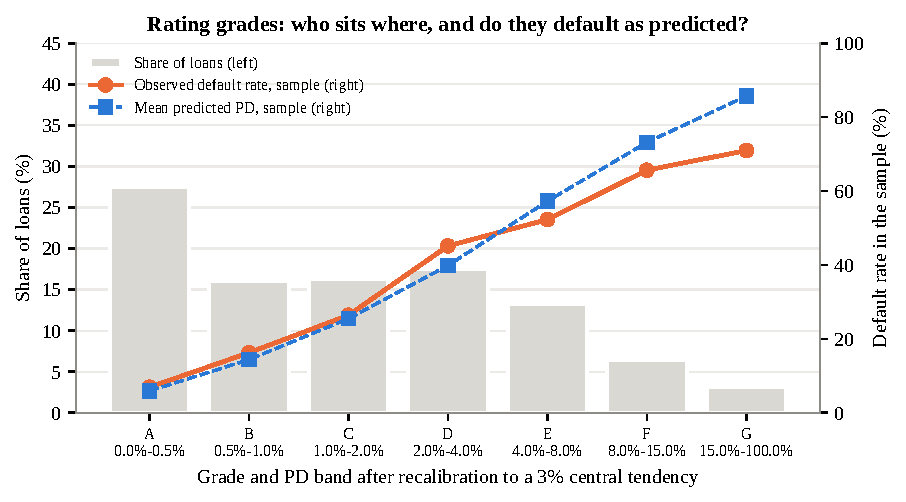
\includegraphics[width=0.86\textwidth]{../figures/fig5_grades.pdf}
\caption{Distribution of loans across grades (bars) and observed against predicted default rates in the sample (lines).}\label{fig:grades}
\end{figure}

\subsection{What the PDs mean for capital}
Figure~\ref{fig:rw} plots the retail risk-weight curve with the seven grades on it. The IRB risk weight stays below the standardised 75\% up to grade~E and exceeds it only for the two riskiest grades, which hold 17\% of the exposure. For the portfolio as a whole, the average IRB risk weight is 53.6\%, or 71.4\% of the standardised requirement. Expected loss is 1.9\% of exposure. It is higher than $3\%\times45\%$ because larger loans tend to be riskier, so the exposure-weighted PD (4.2\%) is above the simple average.

\begin{figure}[htbp]\centering
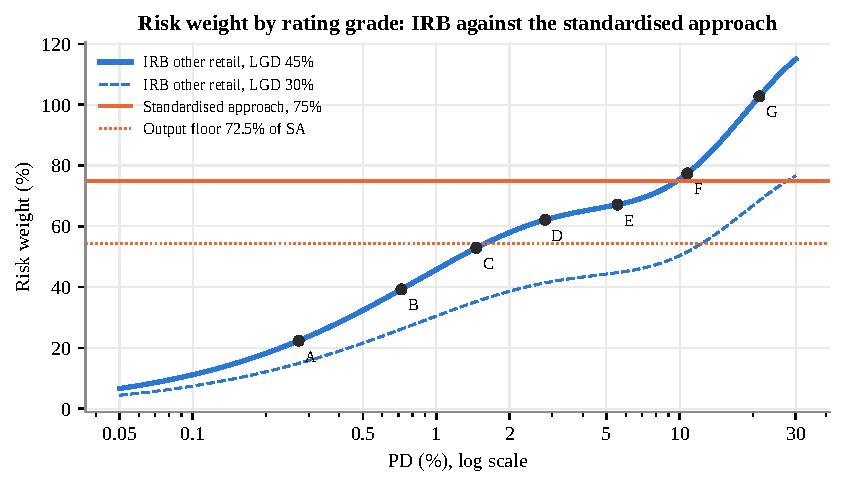
\includegraphics[width=0.86\textwidth]{../figures/fig6_risk_weights.pdf}
\caption{CRR risk-weight function for other retail exposures, with the average PD of each grade (LGD 45\%). The horizontal lines show the standardised 75\% and the fully phased-in output floor.}\label{fig:rw}
\end{figure}

The comparison with the output floor surprised me most. With the floor at 50\%, as in 2025, IRB capital is well above it. At 72.5\%, the level reached in 2030, the floor binds, by a small margin: floored RWA would be DM~1.78 million against DM~1.75 million from the model. Table~\ref{tab:sens} shows that the result does not depend much on my assumptions. In five of the six combinations of portfolio PD and LGD, the fully phased-in floor binds; only a high-risk book (5\% PD, 45\% LGD) escapes it. For a lender with a good-quality consumer portfolio, the advantage of internal models will largely disappear by 2030.

\begin{table}[H]\centering\small
\caption{Capital sensitivity to the assumed portfolio PD and LGD.}\label{tab:sens}
\begin{tabular}{cccccc}
\toprule
Portfolio PD & LGD & Avg IRB RW & IRB / SA & Expected loss & Floor at 72.5\% binds? \\
\midrule
2\% & 30\% & 31.2\% & 0.42 & 0.9\% & Yes \\
2\% & 45\% & 46.8\% & 0.62 & 1.3\% & Yes \\
3\% & 30\% & 35.7\% & 0.48 & 1.3\% & Yes \\
3\% & 45\% & 53.6\% & 0.71 & 1.9\% & Yes \\
5\% & 30\% & 41.9\% & 0.56 & 2.1\% & Yes \\
5\% & 45\% & 62.8\% & 0.84 & 3.1\% & No \\
\bottomrule
\end{tabular}
\end{table}

\section{Discussion}
Put together, the two parts of the analysis tell a fairly consistent story. At the system level, credit quality in Germany is deteriorating faster than in the rest of the EU, especially in commercial real estate and among smaller corporates. At the borrower level, a transparent model can rank risk well, but the capital it produces depends heavily on calibration choices, the portfolio PD and the LGD, that the data cannot pin down. The Bundesbank's warning about low risk weights is about exactly this. So is the output floor, which limits how much capital a bank can save with an optimistic model.

On methods, I expected the machine-learning models to win. They did not. On 1,000 loans, the gain from flexible models is too small to justify losing interpretability, and in a regulated setting, where every rejected applicant can ask why and the AI Act requires human oversight of credit scoring, interpretability has a value of its own. Machine learning is likely to matter more with large datasets and alternative data, but that is a different exercise from the one a student can run on public data.

\section{Limitations}
The borrower-level data are old (according to \citet{groemping2019} they date from the 1970s), small and partly mislabelled, and they describe consumer loans, while the deterioration in the system-level data is concentrated in corporate and real-estate lending. The capital results depend on two assumptions, the 3\% portfolio PD and the 45\% LGD, which is why I report sensitivities rather than a single number. The risk-weight calculation ignores the CRR3 LGD floors for retail, the SME supporting factor and credit-risk mitigation. On the system side, several banking indicators come from secondary reports of EBA data rather than from the original dashboards, and they are point observations rather than consistent time series. Two extensions would help most: re-estimating the models on the corrected South German Credit data, and building a corporate PD model from firm-level balance sheets.

\section{Conclusion}
The credit cycle in Germany has turned. Insolvencies are back at 2014 levels, non-performing loans have grown by almost two thirds since 2021, and German banks now have more loans in Stage~2 than the EU average by a wide margin. On the borrower side, a Weight-of-Evidence logistic scorecard predicts default as well as random forests and gradient boosting (test AUC 0.80) while remaining easy to explain, and its grades are well ordered and mostly well calibrated. Run through the CRR formula, those PDs require about 71\% of the capital of the standardised approach, which is just below the 72.5\% output floor that will apply from 2030. For a typical consumer book, then, internal models will soon save banks very little capital. I think their main use will be in pricing loans and deciding which ones to make.

\medskip
\textit{Code, data and outputs: Python notebook, SQL queries and R script in the accompanying repository.}

\renewcommand{\refname}{References}
\begin{thebibliography}{99}\small\setlength{\itemsep}{2pt}
\bibitem[BaFin(2026)]{bafin2026} Bundesanstalt für Finanzdienstleistungsaufsicht (2026). Risks in Focus 2026: Risks arising from corporate loan defaults. Bonn and Frankfurt.
\bibitem[BCBS(2005)]{bcbs2005} Basel Committee on Banking Supervision (2005). An Explanatory Note on the Basel II IRB Risk Weight Functions. Bank for International Settlements, July 2005.
\bibitem[BKS(2026a)]{bks2026a} Bundesvereinigung Kreditankauf und Servicing e.V. (2026a). Rising NPL ratios in Germany: German NPL ratios against the European trend. Based on the EBA Risk Dashboard Q4 2025.
\bibitem[BKS(2026b)]{bks2026b} Bundesvereinigung Kreditankauf und Servicing e.V. (2026b). NPL Barometer 2026: credit risk concentrates in commercial real estate and SMEs.
\bibitem[Deutsche Bundesbank(2025)]{bbk2025} Deutsche Bundesbank (2025). Financial Stability Review 2025. Frankfurt am Main, 6 November 2025.
\bibitem[Destatis(2023)]{destatis2023} Statistisches Bundesamt (2023). Unternehmen und Arbeitsstätten: Insolvenzverfahren, Mai 2023. Fachserie 2, Reihe 4.1.
\bibitem[Destatis(2026)]{destatis2026} Statistisches Bundesamt (2026). Unternehmensinsolvenzen im Jahr 2025: +10,3\,\% zum Vorjahr. Press release No.~085, 13 March 2026.
\bibitem[ECB(2026)]{ecb2026} European Central Bank (2026). ECB publishes supervisory banking statistics on significant institutions for the fourth quarter of 2025. Press release, 18 March 2026.
\bibitem[EU(2013)]{crr} European Union (2013). Regulation (EU) No 575/2013 on prudential requirements for credit institutions (Capital Requirements Regulation). \textit{Official Journal of the European Union}, L 176.
\bibitem[EU(2024a)]{crr3} European Union (2024a). Regulation (EU) 2024/1623 amending Regulation (EU) No 575/2013 as regards requirements for credit risk, credit valuation adjustment risk, operational risk, market risk and the output floor. \textit{Official Journal of the European Union}.
\bibitem[EU(2024b)]{aiact} European Union (2024b). Regulation (EU) 2024/1689 laying down harmonised rules on artificial intelligence (Artificial Intelligence Act), Annex III. \textit{Official Journal of the European Union}.
\bibitem[Grömping(2019)]{groemping2019} Grömping, U. (2019). South German Credit Data: Correcting a Widely Used Data Set. Reports in Mathematics, Physics and Chemistry, Report 4/2019, Beuth University of Applied Sciences Berlin.
\bibitem[Hofmann(1994)]{hofmann1994} Hofmann, H. (1994). Statlog (German Credit Data). UCI Machine Learning Repository.
\bibitem[Lessmann et al.(2015)]{lessmann2015} Lessmann, S., Baesens, B., Seow, H.-V. and Thomas, L.C. (2015). Benchmarking state-of-the-art classification algorithms for credit scoring: an update of research. \textit{European Journal of Operational Research}, 247(1), 124--136.
\bibitem[PwC(n.d.)]{pwc_crr3} PwC Czech Republic (n.d.). CRR III: what changes for IRB banks. Prague.
\bibitem[Siddiqi(2006)]{siddiqi2006} Siddiqi, N. (2006). \textit{Credit Risk Scorecards: Developing and Implementing Intelligent Credit Scoring}. Wiley, Hoboken.
\end{thebibliography}
\end{document}
